\documentclass[../main/main.tex]{subfiles}

\begin{document}

\newpage
\chapter{Testing}

\section{Iterative Testing}
I have been playtesting the program throughout the development process to find any bugs and fix them accordingly. However, a few issues have required additional measures.

\subsection{Minimax}
Since minimax is recursive algorithm, debugging it has proven a challenge. I have therefore configured the Python \lstinline{logging} library to help collect information on the minimax tree for every function call.

\noindent\verb|base.py|
\lstinputlisting[firstline=27, lastline=52, caption=BaseCPU Method for logging minimax statistics]{../../data/states/game/cpu/base.py}

\subsection{Migrations}
To correct errors made to the \lstinline{games} table, since recreating it would mean deleting all existing games, I have opted to use migrations to fix bugs by editing the table schema, as shown in Section \ref{sec:migrations}.

\section{Unit Tests}
\subsection{Board Evaluator}
To test every aspect of the evaluation function, I have set up some unit tests with custom positions using my editor screen. These positions are designed to test every aspect of the evaluation, along with some obviously imbalanced positions to test the overall accuracy of the evaluation function. All positions are set up to give an advantage to the blue player.

\begin{longtable}[c]{l|l|l|l}
    \toprule
    \textbf{Evaluating} & \textbf{FEN string} & \textbf{Score} & \textbf{Passed}\\
    \midrule
    \endhead

    Material & \verb|sc9/10/10/4paPa4/5Pa4/10/10/9Sa b| & 124 & \checkmark\\
    Position & \verb|sc9/4nanana3/10/10/10/4NaNaNa3/10/9Sa b| & 66 & \checkmark\\
    Mobility & See footnote\footnote{scpapa7/papapa7/papapa1Pa1Pa1Pa1/10/4Pa1Pa1Pa1/10/4Pa1Pa3/9Sa b} & 196 & \checkmark\\
    King Safety & \verb|sc4fa3pa/10/10/10/10/10/10/5FaPa2Sa b| & 3 & \checkmark\\
    Combined & See footnote\footnote{scnc1fcncpbpb3/pa9/pb1pc1rbpa3Pd/1Pc2Pd4Pc/2Pd1RaRb4/10/7Pa2/2PdNaFaNa3Sa b} & 437 & \checkmark\\

    \bottomrule

\caption{Board evaluator test results}
\label{tab:testing-evaluator}
\end{longtable}


\subsection{CPU}
Similarly, to evaluate the strength of my CPU, I have setup some custom positions that I already know the best continuation of, and run each CPU engine on them to test if they can solve it.

\begin{longtable}[c]{l|p{0.45\columnwidth}|l|l}
    \toprule
    \textbf{Description} & \textbf{FEN string} & \textbf{Best Move} & \textbf{Passed}\\
    \midrule
    \endhead

    Mate in 1 & \lstinline|sc9/pafa8/Fa9/10/10/10/10/9Sa b| & Rotate J3 clockwise & \checkmark\\
    Mate in 1 & \lstinline|sc9/10/10/10/8faRb/8FaRb/10/9Sa b| & Move J3 to J2 & \checkmark\\
    Mate in 3 & \lstinline|sc9/10/10/8Ra1/7FaRafa/8RaRa/9Ra/9Sa b| & Move J2 to I1...\footnote{2. \lstinline{Move J4 to J5} 3. \lstinline{Move J3 to I2}} & \checkmark\\
    Mate in 3 & \lstinline|sc5fcnc2/4Pa4Pc/3pb6/2Pc2ra1pb2/10/pb9/7Pa2/2PdNaFa4Sa b| & Move E7 to F7...\footnote{2. \lstinline{Rotate anticlockwise H8} 3. \lstinline{Move F7 to G7}} & \checkmark\\
    Mate in 3 & \lstinline|sc2pdfc5/2Ra1ra5/pa3Pc4Rb/pb1rd1Pdra4/7Rd2/3Ra1Pa4/4Fa5/3PdNaPa3Sa b| & Move J6 to J7...\footnote{2. \lstinline{Move E7 to F8} 3. \lstinline{Move E4 to E5}} & \checkmark\\
    Win Material & \lstinline|sc9/2fa7/5NaPb3/pa2ra1Pd4/3pcnd1pd2Rd/3pc6/10/8FaSa b| & Move F6 to G7...\footnote{2. \lstinline{Move E4 to E3} 3. \lstinline{Move H5 to D4} 4. \lstinline{Move J4 to J3}} & \checkmark\\

    Escape Mate & \lstinline|sc9/10/10/10/8faRb/8FaRb/10/9Sa b| & Move J3 to J2 & \checkmark\\
    \bottomrule

\caption{Iterative Deepening CPU test results}
\label{tab:testing-cpu}
\end{longtable}

% I have also personally played against the CPU engines to gauge its strength in a realistic setting. The results are shown below:

% \begin{longtable}[c]{c|c}
%     \toprule
%     \textbf{Me} & \textbf{CPU}\\
%     \midrule
%     \endhead

%     2 & 5\\

%     \bottomrule

% \caption{Score of me vs CPU (I am very bad)}
% \label{tab:me-cpu}
% \end{longtable}

% \begin{longtable}[c]{c|c}
%     \toprule
%     \textbf{Mr Myslov} & \textbf{CPU}\\
%     \midrule
%     \endhead

%     1 & 6\\

%     \bottomrule

% \caption{Score of Mr Myslov vs CPU (Mr Myslov is even worse)}
% \label{tab:myslov-cpu}
% \end{longtable}

\subsection{Shadow Mapping}
To test the shadow mapping algorithm, I have set up some occluding objects togehter with a light source. Since visuals are subjective, me and my client have deemed the following results to be adequate.

\begin{figure}[H]
    \centering

    \begin{subfigure}[b]{0.3\columnwidth}
    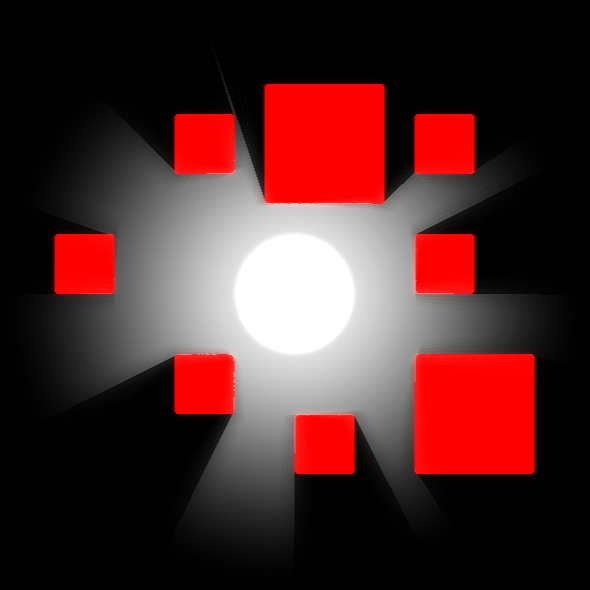
\includegraphics[width=\columnwidth]{../testing/assets/rays_example_1.png}
    \end{subfigure}
    \begin{subfigure}[b]{0.3\columnwidth}
    
\includegraphics[width=\columnwidth]{../testing/assets/rays_example_2.png}
    \end{subfigure}
    \begin{subfigure}[b]{0.3\columnwidth}
    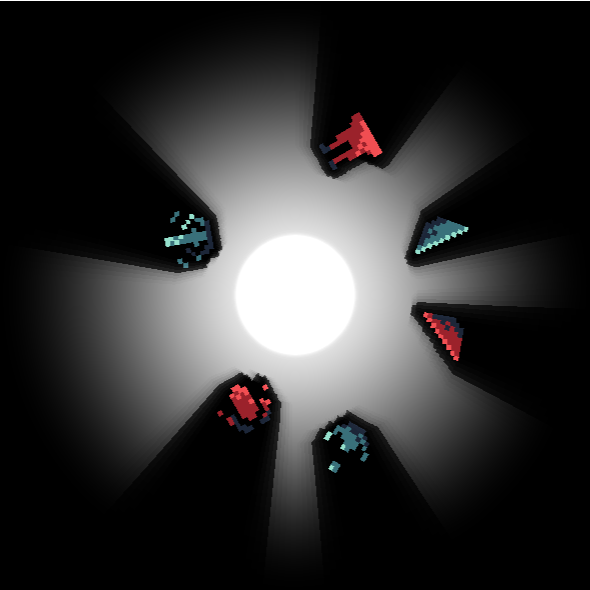
\includegraphics[width=\columnwidth]{../testing/assets/rays_example_3.png}
    \end{subfigure}

    \caption{Shadow mapping algorithm test (softShadow=0.5, radius=0.5)}
    \label{fig:rays-examples}
\end{figure}

\section{Final Tests}
\subsection{Objective 1}
All laser chess game logic should be properly implemented.

\definecolor{light-gray}{HTML}{E9E8E6}
\rowcolors{1}{light-gray}{white}

\begin{longtable}[c]{l|p{0.35\columnwidth}|p{0.35\columnwidth}|l}
    \hiderowcolors
    \toprule
    \textbf{No.} & \textbf{Input} & \textbf{Output} & \textbf{Passed}\\
    \midrule
    \endhead
    \showrowcolors

    6 & Position piece with non-reflecting side facing laser & Piece is destroyed & \checkmark\\
    1 & Laser fires on pyramid & Pyramid reflects laser by 90$^{\circ}$ & \checkmark\\
    2 & Laser fires on scarab & Scarab reflects laser by 90$^{\circ}$ & \checkmark\\
    3 & Laser fires on anubis & Anubis absorbs laser & \checkmark\\
    4 & Move piece as blue player & Active colour switches to red player & \checkmark\\
    5 & Move piece or rotate piece & Laser fires & \checkmark\\
    6 & Fire laser onto pharoah & Pharoah is destroyed and opposite colour wins & \checkmark\\
    8 & Repeat same position three times & Game displays game over screen & \checkmark\\

    \bottomrule

\end{longtable}
\subsection{Objective 2}
Game should process user input correctly.

\begin{longtable}[c]{l|p{0.35\columnwidth}|p{0.35\columnwidth}|l}
    \hiderowcolors
    \toprule
    \textbf{No.} & \textbf{Input} & \textbf{Output} & \textbf{Passed}\\
    \midrule
    \endhead
    \showrowcolors

    8 & Click piece & Overlay appears showing selected piece & \checkmark\\
    9 & Click piece and click outside board & Overlay disappears showing deselected piece & \checkmark\\
    10 & Click piece and click adjacent square & Piece moves to clicked square & \checkmark\\
    11 & Click and hold piece and release over adjacent square & Piece moves to adjacent square & \checkmark\\
    12 & Click piece and press rotate clockwise button & Piece rotates clockwise & \checkmark\\
    12 & Click piece and press rotate anticlockwise button & Piece rotates anticlockwise & \checkmark\\

    \bottomrule

\end{longtable}

\subsection{Objective 3}
Save or load game options should be implemented.

\begin{longtable}[c]{l|p{0.35\columnwidth}|p{0.35\columnwidth}|l}
    \hiderowcolors
    \toprule
    \textbf{No.} & \textbf{Input} & \textbf{Output} & \textbf{Passed}\\
    \midrule
    \endhead
    \showrowcolors

    13 & Click on copy FEN string button in editor or browser screen & Position formatted as FEN string copied to clipboard & \checkmark\\
    14 & Click browser button & Program shows list of past games to be scrolled through & \checkmark\\
    1 & Select time as sorting criterion & Browser updates to show most recent games played & \checkmark\\
    1 & Select descending as ordering criterion & Browser updates to show oldest games played & \checkmark\\
    1 & Click on previous game and click delete button & Selected game is deleted and dissapears & \checkmark\\
    1 & Click on previous game and click review button & Game is displayed in review screen & \checkmark\\
    12 & Enter review screen & Program displays list of past moves, winner and move number& \checkmark\\
    11 & Click on previous button in review screen & Board undoes move & \checkmark\\
    11 & Click on next move button in review screen & Board applies move & \checkmark\\

    \bottomrule

\end{longtable}

\subsection{Objective 4}
Other board game requirements should be implemented.

\begin{longtable}[c]{l|p{0.35\columnwidth}|p{0.35\columnwidth}|l}
    \hiderowcolors
    \toprule
    \textbf{No.} & \textbf{Input} & \textbf{Output} & \textbf{Passed}\\
    \midrule
    \endhead
    \showrowcolors

    13 & Click on draw button & Game ends and shows draw result & \checkmark\\
    14 & Click on resign button & Game ends and shows win result for opponent & \checkmark\\
    15 & Click on timer button to enable timer & Timers appear on the left and decrement every second & \checkmark\\
    16 & Pause the game & Timer stops decrementing & \checkmark\\
    17 & Allow timer to run to zero & Game ends and shows win result for opponent & \checkmark\\

    \bottomrule

\end{longtable}

\subsection{Objective 5}
Game settings and config should be customisable.

\begin{longtable}[c]{l|p{0.35\columnwidth}|p{0.35\columnwidth}|l}
    \hiderowcolors
    \toprule
    \textbf{No.} & \textbf{Input} & \textbf{Output} & \textbf{Passed}\\
    \midrule
    \endhead
    \showrowcolors

    17 & Click on CPU button & Opponent moves are played by minimax CPU & \checkmark\\
    17 & Click on timer button to disable timer & Timer is not shown & \checkmark\\ % Have to also show in video that timer does not run out
    17 & Click on timer duration and input new number & Timer starts with inputted duration & \checkmark\\
    21 & Press starting colour button to set starting colour to red & Starting move is played by the red player & \checkmark\\
    22 & Enter valid FEN string into text input & Board preview updates and game starts with inputted board layout & \checkmark\\
    23 & Enter invalid FEN string into text input & Error message appears & \checkmark\\
    23 & In editor screen, select piece and click on square & Piece placed on square & \checkmark\\
    12 & Click piece and press rotate clockwise button & Piece rotates clockwise & \checkmark\\
    12 & Click piece and press rotate anticlockwise button & Piece rotates anticlockwise & \checkmark\\
    23 & Click empty button & All pieces dissapear (except sphinxes) & \checkmark\\
    23 & Click reset button & Board resets to initial layout & \checkmark\\
    23 & Click confirm button & Switches to config screen with edited FEN string and board preview & \checkmark\\
    23 & Click return button & Switches to config screen with changes discarded & \checkmark\\
    17 & In settings screen, change primary board colour to blue & Alternating board squares appear blue & \checkmark\\
    17 & Change secondary board colour to red & Board squares alternate blue and red & \checkmark\\
    18 & Change display mode to fullscreen & Application window enlarges to fill entire screen & \checkmark\\
    18 & Slide volume thumb to right and left of slider & Music increases and dereases in volume & \checkmark\\
    20 & Toggle particle and shader switches to off position & Particles and shaders are disabled after program restart & \checkmark\\

    \bottomrule

\end{longtable}

\subsection{Objective 6}
Game UI should improve player experience.

\begin{longtable}[c]{l|p{0.35\columnwidth}|p{0.35\columnwidth}|l}
    \hiderowcolors
    \toprule
    \textbf{No.} & \textbf{Input} & \textbf{Output} & \textbf{Passed}\\
    \midrule
    \endhead
    \showrowcolors

    18 & Click on piece & Highlight overlay is rendered on selected square & \checkmark\\
    18 & Click on piece & Circular overlays are rendered on surrounding unoccupied squares & \checkmark\\
    18 & Fire laser on piece & Audio cue plays and piece is visibly destroyed & \checkmark\\
    18 & Fire laser on piece & Piece appears on opponent's piece display & \checkmark\\
    18 & Play a game & Status text updates to display the active player's colour or CPU status & \checkmark\\
    18 & Hover over board, hold the mouse button, click on text input widget & Mouse cursor switches between arrow, open hand, closed hand and I-beam icons & \checkmark\\

    \bottomrule

\end{longtable}

\subsection{Objective 7}
GUI design should be functional and display concise information.

\begin{longtable}[c]{l|p{0.35\columnwidth}|p{0.35\columnwidth}|l}
    \hiderowcolors
    \toprule
    \textbf{No.} & \textbf{Input} & \textbf{Output} & \textbf{Passed}\\
    \midrule
    \endhead
    \showrowcolors

    27 & Click the play button on the main menu screen & Program switches to the config screen & \checkmark\\
    27 & Click the browser button on the main menu screen & Program switches to the browser screen & \checkmark\\
    27 & Click the settings button on the main menu screen & Program switches to the settings screen & \checkmark\\
    28 & Click main menu button & Program switches to the menu screen & \checkmark\\
    29 & Click help button & Help overlay appears & \checkmark\\
    29 & Click quit button & Program quits & \checkmark\\
    31 & Drag program window & Program continues running & \checkmark\\
    30 & Resize program window & GUI Widgets resize continuously & \checkmark\\

    \bottomrule

\end{longtable}

\section{Videos}
Link to video demonstrating final tests: \url{}
\\
Link to video demonstrating unit tests: \url{}

\end{document}